\documentclass[11pt]{article}
\usepackage[a4paper,margin=1in]{geometry}
\usepackage{graphicx}
\usepackage{amsmath}
\usepackage{booktabs}
\usepackage{float}
\usepackage{hyperref}

\title{DSAIT4110 Assignment 2: Model Predictive Control (MPC)\\Analysis Report}
\author{Ioan Hedea}
\date{\today}

\begin{document}
\maketitle

\section{Introduction}
This report summarizes the simulation results for the three MPC modules:
\begin{itemize}
    \item Module 1: prediction and system behavior (open-loop vs closed-loop intuition),
    \item Module 2: constrained MPC behavior under horizon and cost tuning,
    \item Module 3: Tube MPC intuition (nominal vs actual trajectories under bounded disturbances).
\end{itemize}
All figures were generated from the Python scripts in \texttt{mpc/} and saved under \texttt{mpc/figures/}.

\section{Module 1: Prediction and System Behavior}
\subsection{Base Open-Loop Run}
Figure~\ref{fig:m1_base} shows the open-loop trajectories for the default setup
\[
x_0 = [-2,\;3]^\top,\quad u=0.1,\quad d=[0,\;0]^\top.
\]
The state $x_2$ grows approximately linearly, while $x_1$ grows faster due to accumulation through the coupling term in $A$:
\[
x_{1,k+1} = x_{1,k} + 0.1\,x_{2,k}.
\]

\begin{figure}[H]
    \centering
    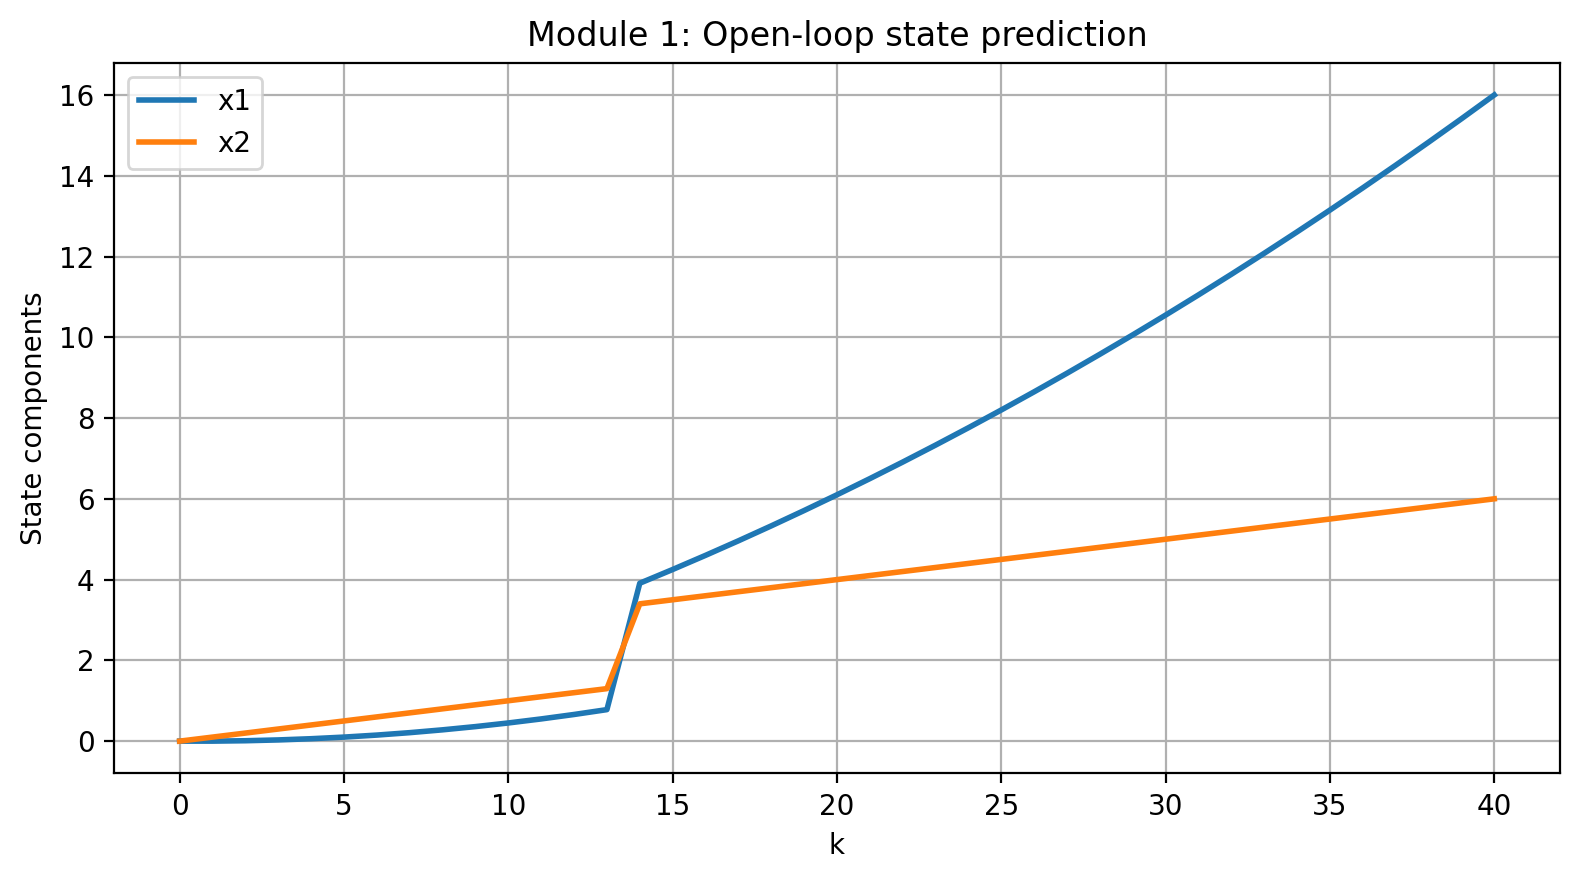
\includegraphics[width=0.88\linewidth]{figures/module1_open_loop.png}
    \caption{Module 1 open-loop prediction (base run).}
    \label{fig:m1_base}
\end{figure}

\subsection{Analysis}
The plot confirms that open-loop behavior is sensitive to initial conditions and model dynamics, since no feedback correction is applied online. In this run, positive $x_2$ keeps integrating into $x_1$, which explains why $x_1$ eventually dominates in magnitude. This supports the motivation for closed-loop control: without feedback, disturbances or state offsets persist and can grow.

\section{Module 2: MPC and Horizon Effects}
\subsection{Base Run ($N_p=3$)}
Figure~\ref{fig:m2_base} shows the constrained MPC closed-loop behavior for
\[
N_p=3,\quad Q=\mathrm{diag}(5,1),\quad R=0.1,\quad u\in[-0.8,0.8].
\]
Both states converge smoothly toward the origin. The applied control remains small and does not hit the input bounds.

\begin{figure}[H]
    \centering
    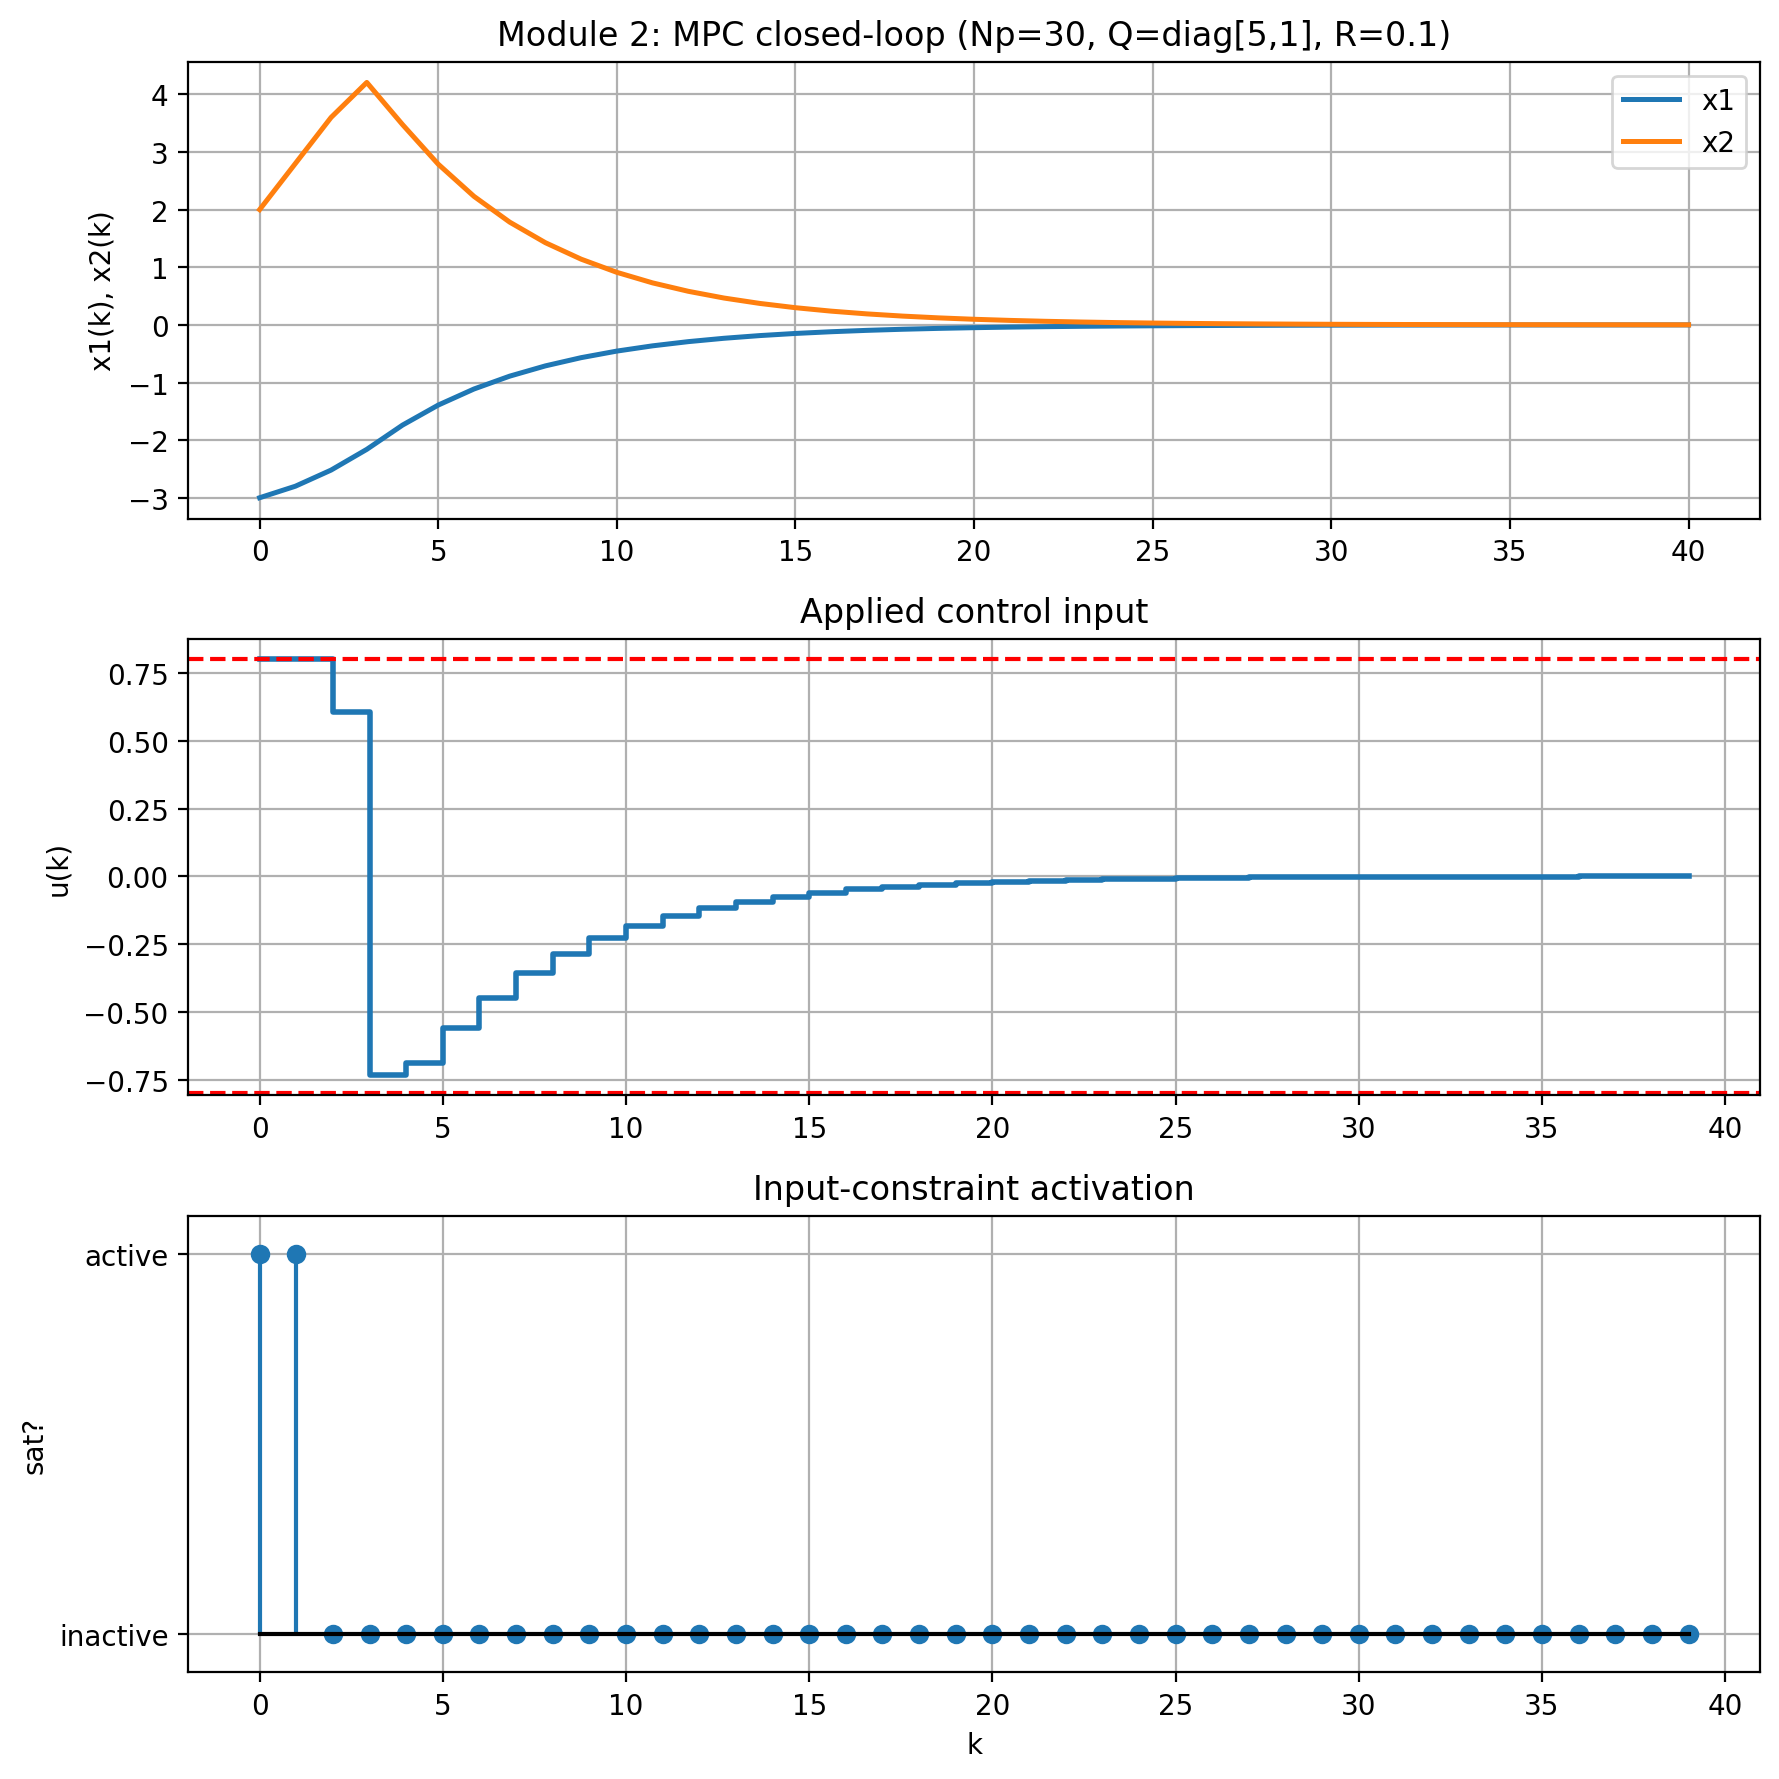
\includegraphics[width=0.96\linewidth]{figures/module2_closed_loop.png}
    \caption{Module 2 constrained MPC: states, input, and input-constraint activity.}
    \label{fig:m2_base}
\end{figure}

\subsection{Analysis}
The baseline run shows a conservative but stable controller response:
\begin{itemize}
    \item states converge monotonically toward zero,
    \item the control sequence is smooth (small step-to-step variation),
    \item the input-constraint activity remains inactive.
\end{itemize}
This is consistent with the quadratic objective where state regulation is weighted more than velocity and input effort is still penalized.

\paragraph{What to add after extra runs.}
To complete the full assignment analysis, include additional runs for:
\begin{itemize}
    \item horizon comparison ($N_p=3,10,30$),
    \item cost tuning (increase $Q$, then increase $R$),
    \item terminal cost comparison ($P$ from DARE).
\end{itemize}
Then discuss convergence speed, smoothness, and saturation differences.

\section{Module 3: Tube MPC Intuition}
\subsection{Base Run (disturbance bound $=0.2$)}
Figure~\ref{fig:m3_base} compares the nominal and disturbed actual trajectories. Circular markers around the nominal path visualize the tube envelope used in the assignment intuition.

\begin{figure}[H]
    \centering
    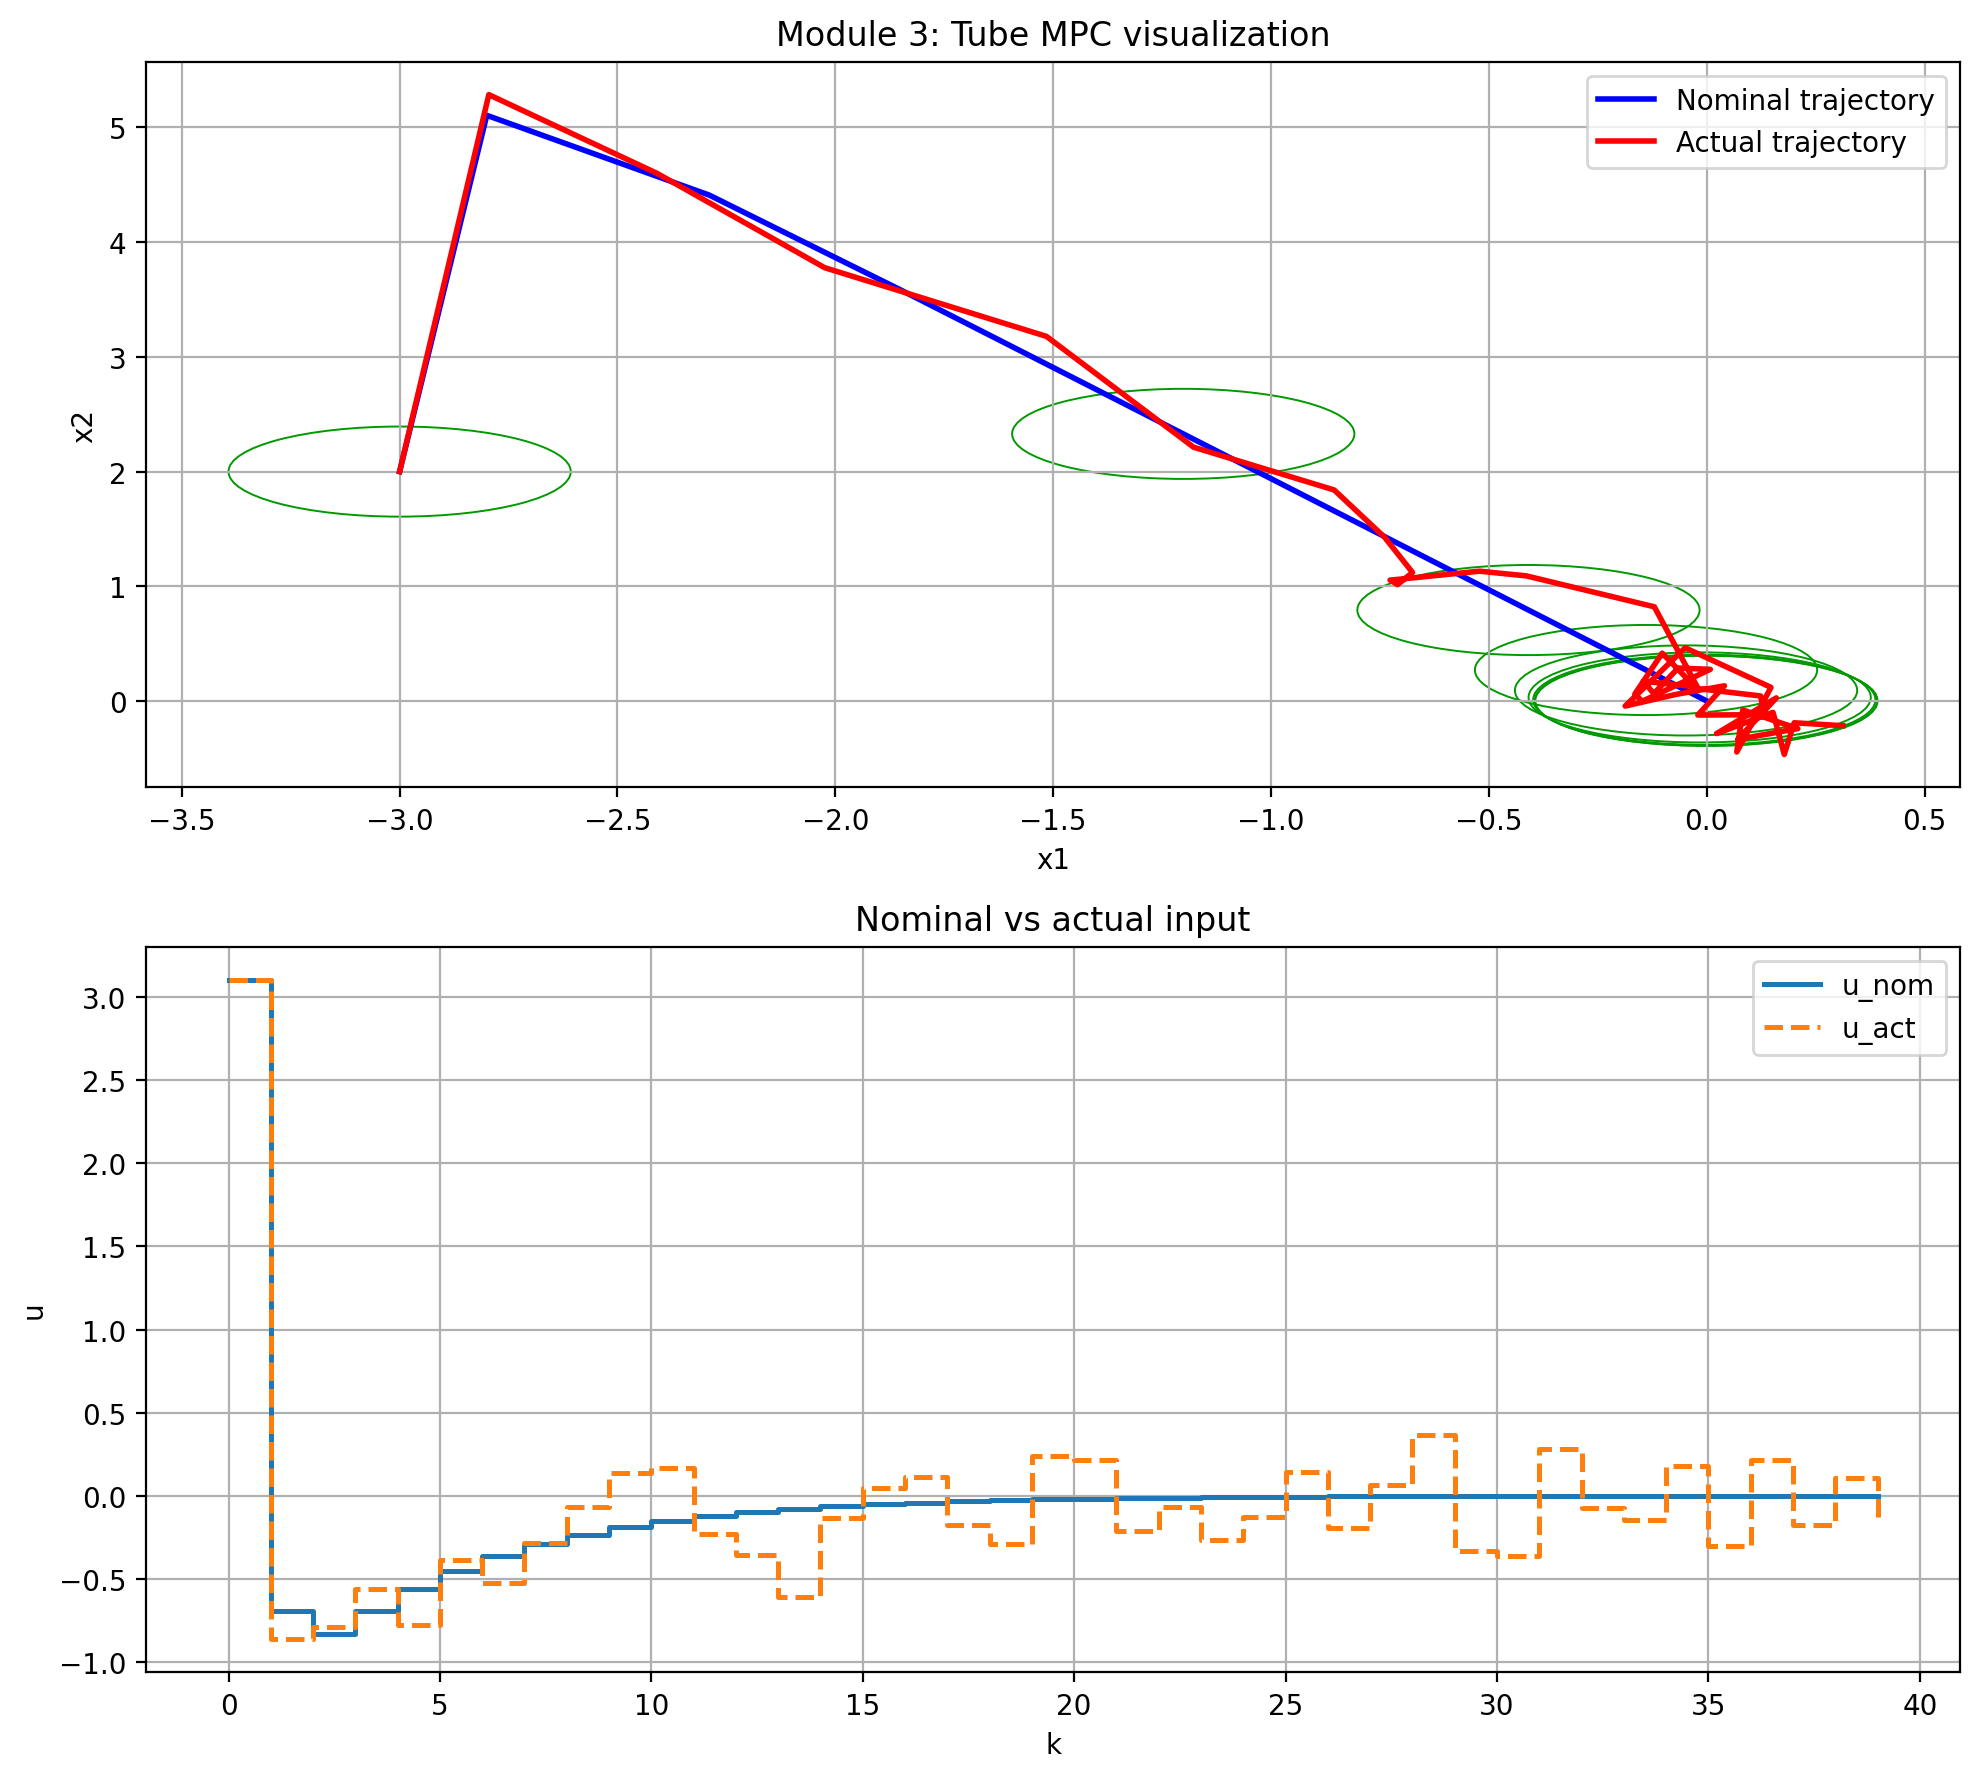
\includegraphics[width=0.96\linewidth]{figures/module3_tube_mpc.png}
    \caption{Module 3 tube MPC visualization: nominal vs actual trajectory and tube cross-sections.}
    \label{fig:m3_base}
\end{figure}

\subsection{Analysis}
The ancillary feedback law
\[
u_k = u_k^{\text{nom}} - K e_k,\quad e_k = x_k - x_k^{\text{nom}}
\]
keeps the disturbed trajectory near the nominal one despite random bounded disturbances. The resulting motion near the origin may still show a mild zig-zag pattern, which is expected from persistent disturbance injection even when $A-BK$ is Schur stable.

\paragraph{What to add after extra runs.}
For full coverage of the module tasks, add experiments with:
\begin{itemize}
    \item multiple disturbance bounds (e.g., $0.1, 0.3, 0.5$),
    \item stronger vs weaker ancillary feedback (via $Q_{\text{error}}, R_{\text{error}}$).
\end{itemize}
Then compare tube width and control aggressiveness.

\section{Conclusion}
Across all modules, the simulations support the lecture concepts:
\begin{itemize}
    \item open-loop prediction is useful but not robust to mismatch/disturbances,
    \item MPC provides structured closed-loop regulation with explicit cost/constraint trade-offs,
    \item tube-based feedback improves robustness by separating nominal planning from disturbance rejection.
\end{itemize}

\end{document}
